\documentclass[11pt]{article}
\usepackage[a4paper,margin=27mm]{geometry}
\usepackage[T1]{fontenc}
\usepackage{lmodern}
\usepackage{amsmath,amssymb,amsthm,mathtools}
\usepackage{microtype,booktabs,array,graphicx}
\usepackage[shortlabels]{enumitem}
\usepackage[dvipsnames]{xcolor}
\usepackage{hyperref}
\usepackage[nameinlink,noabbrev]{cleveref}
\usepackage{fancyhdr}
\hypersetup{colorlinks=true,linkcolor=MidnightBlue,citecolor=MidnightBlue,urlcolor=MidnightBlue,
  pdftitle={Uniform rank and joint-defect laws for rectangular symplectic blocks},
  pdfauthor={Research note extending the ProveIt development}}
\pagestyle{fancy}
\fancyhf{}
\fancyhead[L]{\small Rectangular symplectic blocks}
\fancyhead[R]{\small 27 November 2026}
\fancyfoot[C]{\thepage}
\setlength{\headheight}{14pt}
\setlength{\emergencystretch}{2em}
\allowdisplaybreaks[2]
\newtheorem{theorem}{Theorem}[section]
\newtheorem{proposition}[theorem]{Proposition}
\newtheorem{lemma}[theorem]{Lemma}
\newtheorem{corollary}[theorem]{Corollary}
\theoremstyle{definition}
\newtheorem{definition}[theorem]{Definition}
\newtheorem{remark}[theorem]{Remark}
\newcommand{\F}{\mathbb F_q}
\newcommand{\E}{\mathbb E}
\newcommand{\Pbb}{\mathbb P}
\newcommand{\Law}{\mathcal L}
\newcommand{\TV}{d_{\mathrm{TV}}}
\newcommand{\Mat}{\operatorname{Mat}}
\newcommand{\Alt}{\operatorname{Alt}}
\newcommand{\Sp}{\operatorname{Sp}}
\newcommand{\GL}{\operatorname{GL}}
\newcommand{\rank}{\operatorname{rank}}
\newcommand{\nul}{\operatorname{null}}
\newcommand{\rad}{\operatorname{rad}}
\newcommand{\Cov}{\operatorname{Cov}}
\newcommand{\qbin}[2]{\genfrac{[}{]}{0pt}{}{#1}{#2}_q}
\newcommand{\normone}[1]{\left\|#1\right\|_1}
\newcommand{\trans}{\mathsf T}
\newcommand{\ind}{\mathbf 1}
\newcommand{\eps}{\varepsilon}
\newcommand{\gitsha}{\texttt{497c1844e71393df41914f5b783d5dc9a618eb61}}
\newcommand{\srcid}[1]{{\footnotesize\ttfamily #1}}
\title{\vspace{-1em}\textbf{Uniform rank and joint-defect laws\\for rectangular symplectic blocks}\\[0.5em]
\large Persistent matrix dependence, vanishing rank information,\\and a sharp independence theorem}
\author{Research note extending the ProveIt development}
\date{27 November 2026}

\begin{document}
\maketitle
\begin{abstract}
Let \(A\) be an \(a\times b\) block of a uniform symplectic transformation,
where source and target are complementary nondegenerate spaces over \(\F\).
For all positive even \(a\ge b\), we obtain signed first-order expansions for
the nullity law of \(A\), the nullity of the translated Gram form
\(D(U)=J_b-U^{\trans}J_aU\) of an independent-entry matrix \(U\), and the
centered joint law of the nullities of \(U\) and \(D(U)\).
These signed-law remainders are \(O_q(q^{-a-b})\), uniformly in the
gap \(a-b\). In particular, the rank testing distance is
\[
 \TV(\rank A,\rank U)
 =\frac{\gamma_\infty}{(q-1)\gamma_{a-b}}\,q^{-a}
   +O_q(q^{-a-b}),\qquad
 \gamma_r=\prod_{i=1}^r(1-q^{-i}).
\]
The rank of \(U\) and the rank of \(D(U)\) are asymptotically independent with
an explicit signed correction and sharp constant. Their two full-rank
indicators retain the entire first-order dependence.
Meanwhile, the full matrix laws stay a positive distance apart, with a
limit independent of the aspect ratio and an explicit symmetric correction.
This resolves the fixed-positive-gap case singled out in the
ProveIt GRH transfer article. Exact likelihoods and classical complement
counts are credited as inputs; the principal extension is the uniform
signed-law analysis, especially the joint theorem.
All proofs are unconditional and valid in characteristic two.
\end{abstract}

\section{Source, question, and contribution}\label{sec:source}

The starting point is the directory
\href{https://github.com/VladimirReshetnikov/ProveIt/tree/497c1844e71393df41914f5b783d5dc9a618eb61/Analysis/GeneralizedRiemannHypothesis}{\texttt{Analysis/GeneralizedRiemannHypothesis}}
at revision \gitsha.
Its article collects consequences of Dirichlet GRH and transfers of methods
from its proof \cite{ProveIt}. The source development contains finite-group
compression and kernel-counting arguments; for example,
\srcid{New/Spanning/SecondMoment/PositiveType.lean} bounds singular
compressions using additive characters and a second moment \cite{GRHSource}.
The article subsequently studies uniform symplectic compressions by exact
orbit counts. The present paper extends that finite-field branch of the
research. Its proof uses neither a zero hypothesis nor an unverified
arithmetic estimate.

The specific starting question is \srcid{spn:q:symplectic},
\emph{Growing symplectic compressions}, in \texttt{Article/sections/spn.tex}.
It explicitly leaves the fixed positive difference \(a-b\) unresolved for
complementary nondegenerate frames. The article already contains the exact
likelihood, the square case, and a limiting result when the rectangle
becomes increasingly tall. These facts are the baseline, not claims of this paper.

\begin{center}
\small
\begin{tabular}{>{\raggedright\arraybackslash}p{0.31\linewidth}>{\raggedright\arraybackslash}p{0.59\linewidth}}
\toprule
Existing result & Extension proved here\\
\midrule
Exact likelihood and residual-singularity test,
\srcid{spn:thm:balanced}
& Reproved for completeness; combined with uniform expansions.\\[3pt]
Square signed rank and defect laws,
\srcid{spn:thm:square-block} and
\srcid{spn:thm:defect-universality}
& Signed laws for every even rectangular gap, with a remainder
\(O_q(q^{-a-b})\) that stays smaller than the main term uniformly.\\[3pt]
Increasingly tall blocks,
\srcid{spn:thm:nondeg-blind}
& Sharp rank asymptotics in every aspect ratio, including a fixed positive gap.\\[3pt]
Exact moments and a route to joint counts in the square case
& A centered joint-law expansion, a sharp independence distance,
and an asymptotically optimal two-bit test.\\
\bottomrule
\end{tabular}
\end{center}

The classical independent-entry rectangular and alternating rank laws are
treated by Fulman and Goldstein \cite{FG}. De Boeck and Van de Voorde give
exact complementary-subspace counts \cite{DBV}; those counts supply an
independent short route to our full-matrix companion asymptotic.
Pott, Schmidt and Zhou study exact rank intersections for pairs of
alternating forms \cite{PSZ}. The bounded literature search for this note
did not locate the uniform signed rank, translated-defect, or centered
joint expansions stated below. This supports novelty relative to the
inspected sources; it does not certify global priority.

\section{Model and main theorems}\label{sec:main}

Fix a prime power \(q\). An alternating matrix means a matrix \(H\) with
\(H^{\trans}=-H\) and zero diagonal; the diagonal condition is retained in
characteristic two. For every even \(D\), fix a nonsingular alternating
matrix \(J_D\) of size \(D\). Let \(a\ge b\ge2\) be even and let \(g\) be
uniform in the symplectic group of
\[
 V=(\F^a,J_a)\perp(\F^b,J_b).
\]
Apply \(g\) to the coordinate frame of the second summand and write its
image as \(\binom A B\). Thus \(A\in\Mat_{a,b}(\F)\),
\(B\in\Mat_b(\F)\), and
\begin{equation}\label{eq:gram-condition}
 A^{\trans}J_aA+B^{\trans}J_bB=J_b.
\end{equation}
The frame is uniform among all solutions of \eqref{eq:gram-condition}.
Let \(U\) be uniform in \(\Mat_{a,b}(\F)\), with independent entries, and
let \(T_b\) be uniform in \(\Alt_b(\F)\). Put
\[
\begin{gathered}
 D(M)=J_b-M^{\trans}J_aM,\quad
 K_M=b-\rank M,\quad L_M=\nul D(M),\\
 d=a-b,\quad u=q^{-a},\quad v=q^{-b}.
\end{gathered}
\]
For the joint theorem \(K=K_U\) and \(L=L_U\).

For a signed measure \(\rho\) on a countable set,
\(\normone{\rho}=\sum_x|\rho(x)|\). Total variation between probability
laws is \(\TV(P,Q)=\tfrac12\normone{P-Q}\), equivalently the largest
difference in probabilities of an event.

Define
\begin{equation}\label{eq:products}
 \gamma_r=\prod_{i=1}^r(1-q^{-i}),\qquad
 \eta_r=\prod_{i=1}^r(1-q^{-2i}),\qquad
 \theta_r=\prod_{i=1}^r(1-q^{-(2i-1)}).
\end{equation}
Empty products are one. Their positive infinite limits satisfy
\(\gamma_\infty=\eta_\infty\theta_\infty\).
The classical limiting nullity laws are
\begin{align}
 \pi_d(k)&=\frac{\gamma_\infty q^{-k(k+d)}}{\gamma_k\gamma_{k+d}}
       &&(k\ge0),\label{eq:pi}\\
 \lambda(2k)&=\frac{\theta_\infty q^{-k(2k-1)}}{\gamma_{2k}},
 &\lambda(2k+1)&=0.\label{eq:lambda}
\end{align}
We use the explicit signed sequences
\begin{equation}\label{eq:signed}
 \xi_d(k)=\frac{1+q^{-d}-q^k}{q-1}\,\pi_d(k),
 \qquad
 \zeta(k)=\frac{q+1-q^k}{q^2-1}\,\lambda(k).
\end{equation}
They both have total mass zero. Each has its only strictly positive mass
at zero; some other coefficients may vanish.

\begin{theorem}[Uniform signed marginal laws]\label{thm:marginals}
For each \(q\) there is \(C_q<\infty\) such that, for every positive even
\(a\ge b\),
\begin{align}
 \normone{\Law(K_A)-\Law(K_U)-q^{-b}\xi_d}
       &\le C_q q^{-a-b},\label{eq:rank-expansion}\\
 \normone{\Law(L_U)-\Law(\nul T_b)-q^{-a}\zeta}
       &\le C_q q^{-a-b}.\label{eq:defect-expansion}
\end{align}
In particular,
\begin{align}
 \TV(\rank A,\rank U)
   &=\frac{\gamma_\infty}{(q-1)\gamma_d}\,q^{-a}
      +O_q(q^{-a-b}),\label{eq:rank-tv}\\
 \TV(L_U,\nul T_b)
   &=\frac{q\theta_\infty}{q^2-1}\,q^{-a}
      +O_q(q^{-a-b}).\label{eq:defect-tv}
\end{align}
All error constants depend only on \(q\), not on \(a,b\), or \(d\).
\end{theorem}

The coefficient in \eqref{eq:rank-tv} is bounded between
\(\gamma_\infty/(q-1)\) and \(1/(q-1)\). Thus its relative error is
\(O_q(q^{-b})\), even if \(d\) grows arbitrarily quickly with \(b\).
A bound \(O_q(q^{-2b})\) in place of the stated remainder would not have
this property.

\begin{theorem}[Sharp joint asymptotic independence]\label{thm:joint}
Let \(P_{a,b}=\Law(K,L)\), and let \(P_K,P_L\) denote its actual finite
marginal laws. Uniformly for all positive even \(a\ge b\),
\begin{equation}\label{eq:joint-expansion}
 \normone{P_{a,b}-P_K\otimes P_L
            +q^{-b}(q^2-1)\xi_d\otimes\zeta}
     \le C_q q^{-a-b}.
\end{equation}
Consequently,
\begin{equation}\label{eq:joint-tv}
 \TV(P_{a,b},P_K\otimes P_L)
   =\frac{2q\theta_\infty\gamma_\infty}{(q-1)\gamma_d}\,q^{-a}
      +O_q(q^{-a-b}).
\end{equation}
\end{theorem}

The centering in this theorem uses the true finite marginals. It
therefore measures dependence itself, rather than a combination of
dependence and the convergence of the two marginal distributions.

\begin{corollary}[Two Boolean observations retain the leading dependence]
\label{cor:xor}
Let \(E=\{K=0\}\), \(F=\{L=0\}\), and
\(X=(E\cap F^c)\cup(E^c\cap F)\). Then
\begin{align}
 \Cov(\ind_E,\ind_F)
   &=-\frac{q\theta_\infty\gamma_\infty}{(q-1)\gamma_d}\,q^{-a}
       +O_q(q^{-a-b}),\label{eq:covariance}\\
 P_{a,b}(X)-(P_K\otimes P_L)(X)
   &=\TV(P_{a,b},P_K\otimes P_L)+O_q(q^{-a-b}).\label{eq:xor}
\end{align}
Thus the test that exactly one of \(U\) and \(D(U)\) has full rank is
asymptotically optimal for detecting their dependence. Exact optimality
at every finite size is not asserted.
\end{corollary}

\begin{theorem}[Persistent full-matrix discrepancy]\label{thm:full}
Put
\[
 \alpha_{a,b}=\frac{\eta_{a/2}\eta_{b/2}}{\eta_{(a+b)/2}},\qquad
 \Delta_q=\theta_\infty(1-\eta_\infty),\qquad
 c_q=\frac{\theta_\infty\{q-(q+1)\eta_\infty\}}{q^2-1}<0.
\]
At every finite size, the event \(D(M)\) singular is an optimal test
between \(A\) and \(U\), and
\begin{equation}\label{eq:full-exact}
 \TV(A,U)=(1-\alpha_{a,b})\,\Pbb(D(U)\text{ nonsingular}).
\end{equation}
Moreover,
\begin{equation}\label{eq:full-asymp}
 \TV(A,U)=\Delta_q+c_q(q^{-a}+q^{-b})
                  +O_q((q^{-a}+q^{-b})^2).
\end{equation}
Hence \(\TV(A,U)\to\Delta_q>0\) whenever both dimensions tend to
infinity, in every aspect ratio.
\end{theorem}

The exact test in \cref{thm:full} is inherited from the article. The
new uniform analysis gives a common treatment of the dimensional
regimes and combines it with \cref{thm:marginals,thm:joint}.
For \(q=2\),
\[
 \Delta_2=0.1306343467085051764310563857\ldots.
\]
In an equal-prior decision problem, observing the whole matrix therefore
has limiting optimal success probability
\((1+\Delta_2)/2=0.565317173354252588\ldots\).
Any rank-only procedure has success tending to \(1/2\), at the sharp
rate \eqref{eq:rank-tv}.

Our orientation \(a\ge b\) loses no full-matrix or rank generality.
Inversion in the symplectic group sends an off-diagonal block to its
transpose multiplied on both sides by fixed invertible matrices.
After exchanging the two summands, this identifies the opposite
rectangular model. Both rank and total variation are unchanged.
The statements concerning \(D(U)\) use the displayed orientation.

\section{Exact finite counts}\label{sec:counting}

The exact formulas in this section are finite identities. They provide
both the starting point for the asymptotic proof and a direct method for
evaluating the distributions.

\subsection{Isometric embeddings and subspaces}

Let \(E_D(j,s)\) be the number of isometric injections of a fixed
\(j\)-dimensional alternating space of rank \(2s\) into a nondegenerate
alternating space of even dimension \(D\). Set
\begin{equation}\label{eq:Phi}
 \Phi_D(j,s)=
 \begin{cases}
 \displaystyle\prod_{r=D/2-j+s+1}^{D/2}(1-q^{-2r}),
                 &j-s\le D/2,\\
 0,              &j-s>D/2.
 \end{cases}
\end{equation}

\begin{lemma}[Prescribed-Gram embeddings]\label{lem:embeddings}
For \(0\le2s\le j\),
\begin{equation}\label{eq:embedding}
 E_D(j,s)=q^{Dj-\binom j2}\Phi_D(j,s).
\end{equation}
The number \(N_D(j,s)\) of \(j\)-subspaces of a symplectic \(D\)-space
with restricted rank \(2s\) is
\begin{equation}\label{eq:types}
 N_D(j,s)=
 \frac{E_D(j,s)}
 {|\Sp_{2s}(\F)|\,|\GL_{j-2s}(\F)|\,q^{2s(j-2s)}}.
\end{equation}
\end{lemma}

\begin{proof}
Choose a symplectic basis of the nondegenerate part and then a basis of
its radical. Embedding the \(s\) ordered hyperbolic pairs gives
\[
 \prod_{i=0}^{s-1}(q^{D-2i}-1)q^{D-2i-1}
\]
choices. In the remaining nondegenerate space of dimension \(D-2s\),
an ordered isotropic radical frame of size \(j-2s\) has
\[
 \prod_{i=0}^{j-2s-1}(q^{D-2s-i}-q^i)
\]
choices. Such a frame exists precisely when \(j-s\le D/2\).
Collecting the powers of \(q\) gives \eqref{eq:embedding}.

The automorphisms of a form with nondegenerate part of dimension \(2s\)
and radical dimension \(r=j-2s\) have order
\(|\Sp_{2s}(\F)|\,|\GL_r(\F)|q^{2sr}\).
Dividing the number of injective realizations by this order gives
\eqref{eq:types}. Symplectic Gram--Schmidt also extends every isometry
between these subspaces to an ambient isometry: extend a radical basis
by dual partners, then complete a symplectic basis. This argument
requires no division by two.
\end{proof}

\subsection{Likelihood and optimal event}

For \(k\ge0\), define
\begin{equation}\label{eq:F}
 F_q(k)=\sum_{r=k}^{2k}\qbin{2k}{r}
                 \frac{q^{-r(r+1)/2}}{\eta_{r-k}}.
\end{equation}

\begin{proposition}[Exact residual likelihood]\label{prop:likelihood}
For any \(M\in\Mat_{a,b}(\F)\), if \(\nul D(M)=2k\), then
\begin{equation}\label{eq:likelihood}
 q^{ab}\Pbb(A=M)=\alpha_{a,b}F_q(k).
\end{equation}
This likelihood is smaller than one for \(k=0\), and larger than one
for every \(k\ge1\).
\end{proposition}

\begin{proof}
A prescribed \(M\) is completed by the square matrices \(B\) satisfying
\(B^{\trans}J_bB=D(M)\).
Their kernels lie in the \(2k\)-dimensional radical of \(D(M)\).
If such a kernel has dimension \(r\), the quotient has dimension \(b-r\)
and rank \(b-2k\), so it embeds in dimension \(b\) if and only if
\(k\le r\le2k\). There are \(\qbin{2k}{r}\) kernels and
\[
 E_b(b-r,b/2-k)
   =q^{b(b+1)/2-r(r+1)/2}\frac{\eta_{b/2}}{\eta_{r-k}}
\]
isometric embeddings for each quotient.
The total number of frames satisfying \eqref{eq:gram-condition} is
\[
 E_{a+b}(b,b/2)
 =q^{(a+b)b-\binom b2}\frac{\eta_{(a+b)/2}}{\eta_{a/2}}.
\]
Every such frame is injective because its Gram matrix \(J_b\) is
nonsingular, and the symplectic group is transitive on these frames.
Dividing the completion count by this frame count and multiplying by
\(q^{ab}\) gives \eqref{eq:likelihood}.

For \(k=0\), \(F_q(0)=1\), and \(\alpha_{a,b}<1\):
the \(b/2\) factors of
\(\eta_{(a+b)/2}/\eta_{a/2}\) have strictly larger indices than those of
\(\eta_{b/2}\).
Also
\[
 \alpha_{a,b}\ge\eta_\infty
       >1-\sum_{r\ge1}q^{-2r}
       =\frac{q^2-2}{q^2-1}.
\]
For \(k=1\), direct summation gives
\(F_q(1)=1+q/(q^2-1)\), and
\[
 \frac{q^2-2}{q^2-1}
      \left(1+\frac q{q^2-1}\right)-1
   =\frac{q^3-q^2-2q+1}{(q^2-1)^2}>0
       \qquad(q\ge2).
\]
For \(k\ge2\), the term \(r=k\) alone yields
\[
 \alpha_{a,b}F_q(k)
 \ge\eta_\infty\qbin{2k}{k}q^{-k(k+1)/2}
 \ge\eta_\infty q^{k(k-1)/2}>1.
\]
All excess mass is therefore on singular residuals. On nonsingular
residuals the deficit is the constant \(1-\alpha_{a,b}\), proving
\eqref{eq:full-exact}.
\end{proof}

\subsection{Exact marginal moments}

Gaussian binomial coefficients count subspaces:
\(\qbin{n}{j}\) is the number of \(j\)-subspaces of \(\F^n\).
For \(0\le j\le b\), define
\[
 \mu_j=\E\qbin{K_A}{j},\quad
 \mu_j^0=\E\qbin{K_U}{j},\quad
 \nu_j=\E\qbin{L_U}{j},\quad
 \nu_j^0=\E\qbin{\nul T_b}{j}.
\]

\begin{lemma}[Kernel and defect moments]\label{lem:moments}
One has
\begin{align}
 \mu_j
 &=\sum_s N_b(j,s)\frac{E_b(j,s)}{E_{a+b}(j,s)},
 & \mu_j^0&=\qbin b j q^{-aj},\label{eq:rank-moments-raw}\\
 \nu_j
 &=q^{-(a+b)j+j^2}\sum_sN_b(j,s)E_a(j,s),
 & \nu_j^0&=\qbin b j q^{-bj+j(j+1)/2}.
 \label{eq:defect-moments-raw}
\end{align}
\end{lemma}

\begin{proof}
For the first formula, sum over \(j\)-subspaces \(W\) of the source.
If \(W\) has restricted rank \(2s\), its image under the random frame
is uniform among \(E_{a+b}(j,s)\) isometric injections.
The condition \(AW=0\) says that this image lies in the hidden
\(b\)-dimensional summand, allowing \(E_b(j,s)\) injections.
For the independent matrix \(U\), killing \(W\) imposes \(aj\)
independent scalar conditions.

For the defect, suppose \(W\subseteq\ker D(U)\). If \(x\in W\) and
\(Ux=0\), then for every \(y\in\F^b\),
\[
 x^{\trans}J_by=(Ux)^{\trans}J_a(Uy)=0,
\]
so \(x=0\). Thus \(U|_W\) is an isometric injection, with \(E_a(j,s)\)
choices. After fixing it, each of the \(b-j\) remaining basis vectors
has \(j\) independent prescribed pairings, and hence \(q^{a-j}\)
possible images. Divide by \(q^{ab}\) and sum over \(W\).
Finally, an alternating \(b\times b\) matrix that kills a given
\(j\)-space has \(bj-j(j+1)/2\) independent entries prescribed to zero.
\end{proof}

Let \(H\) be uniform in \(\Alt_j(\F)\), and write \(\rank H=2s\).
Define
\[
 m_{j,d}=\frac{q^{-j(j+d)}}{\gamma_j},\qquad
 m'_j=\frac{q^{-j(j-1)/2}}{\gamma_j}.
\]
The probability that \(H\) has rank \(2s\) is
\[
 \frac{|\GL_j(\F)|}
 {q^{\binom j2}|\Sp_{2s}(\F)|
       |\GL_{j-2s}(\F)|q^{2s(j-2s)}}.
\]
Substituting Lemma~\ref{lem:embeddings} into the moment formulas gives the
useful common normalization
\begin{equation}\label{eq:unified}
 \begin{aligned}
 \mu_j&=m_{j,d}\E_H\frac{\Phi_b(j,s)^2}{\Phi_{a+b}(j,s)},
 &\quad \mu_j^0&=m_{j,d}\E_H\Phi_b(j,s),\\
 \nu_j&=m'_j\E_H\{\Phi_b(j,s)\Phi_a(j,s)\},
 &\quad \nu_j^0&=m'_j\E_H\Phi_b(j,s).
 \end{aligned}
\end{equation}
Every denominator in this formula is nonzero: \(j\le b\le a\)
implies \(j-s\le(a+b)/2\).

\subsection{The reference distributions}

Counting maps by their kernels gives
\begin{equation}\label{eq:finite-iid}
 \Pbb(K_U=k)
 =q^{-k(k+d)}
       \frac{\gamma_a\gamma_b}
       {\gamma_k\gamma_{d+k}\gamma_{b-k}}
       \quad(0\le k\le b).
\end{equation}
Similarly, choose the radical of an alternating form and then a
nondegenerate form on its quotient:
\begin{equation}\label{eq:finite-alt}
 \Pbb(\nul T_b=2k)
   =q^{-k(2k-1)}
       \frac{\gamma_b}{\gamma_{2k}\eta_{b/2-k}}
       \quad(0\le k\le b/2).
\end{equation}
Odd nullities have probability zero. These formulas imply
\eqref{eq:pi} and \eqref{eq:lambda}; the quadratic tails justify passage to each
fixed Gaussian moment. Therefore
\begin{equation}\label{eq:limit-moments}
 \sum_k\qbin k j\pi_d(k)=m_{j,d},
 \qquad
 \sum_k\qbin k j\lambda(k)=m'_j.
\end{equation}
They also prove that both limiting sequences have total mass one.
No convergence of a moment series is being used without a tail bound.


\section{Uniform marginal expansions}\label{sec:marginal-proof}

Throughout the proof, constants denoted \(C_q\) may change from line to
line but depend only on \(q\). The estimates below also explain why
the error is uniform when \(d=a-b\) grows.

\subsection{Expansion of the embedding product}

For an alternating \(j\times j\) form \(H\) of rank \(2s\), put
\[
 W(H)=\frac{q^{2(j-s)}-1}{q^2-1},
 \qquad Q_j=\frac{q^j-1}{q-1}.
\]

\begin{lemma}[Uniform product estimates]\label{lem:products}
Including the zero convention for infeasible embeddings,
\begin{align}
 0\le\Phi_D(j,s)&\le1,\qquad
 |\Phi_D(j,s)-1|\le q^{-D}W(H),\label{eq:product-first}\\
 \Phi_D(j,s)
   &=1-q^{-D}W(H)+O_q(q^{-2D}q^{4j}).\label{eq:product-second}
\end{align}
For \(j\le b\le a\), \(\Phi_{a+b}(j,s)\ge\eta_\infty\).
Moreover,
\begin{equation}\label{eq:Wmean}
 \E_HW(H)=Q_j.
\end{equation}
\end{lemma}

\begin{proof}
On the feasible range, the sum of the deficits of the factors in
\(\Phi_D\) is exactly
\[
 \sum_{r=D/2-j+s+1}^{D/2}q^{-2r}=q^{-D}W(H).
\]
For nonnegative \(t_i\le1\), their product satisfies
\[
 0\le \prod_i(1-t_i)-1+\sum_i t_i
       \le\frac12\left(\sum_i t_i\right)^2.
\]
For example, interpret the \(t_i\) as the probabilities of independent
events and apply the first two inclusion--exclusion bounds.
This proves the two estimates on the feasible range.
If \(j-s>D/2\), then \(q^{-D}W(H)\ge1\);
the estimates follow from \(\Phi_D=0\) and the quadratic bound
\(t-1\le t^2\) for \(t\ge1\).
The lower bound for \(\Phi_{a+b}\) follows because it is a finite
product of a subset of the factors of \(\eta_\infty\).

For \(j\ge1\), a fixed nonzero vector is in the radical of a uniform
alternating \(H\) with probability \(q^{-(j-1)}\).
Thus
\[
 \E_H q^{\nul H}=1+(q^j-1)q^{1-j}.
\]
Since \(2(j-s)=j+\nul H\), inserting this expression into the
definition of \(W\) proves \eqref{eq:Wmean}. The case \(j=0\) is
immediate.
\end{proof}

Use \(\Phi_b^2-\Phi_b=(\Phi_b-1)+(\Phi_b-1)^2\) rather than
multiplying two potentially large error estimates. Together with
\(\Phi_{a+b}\ge\eta_\infty\), this gives
\[
 \frac{\Phi_b^2}{\Phi_{a+b}}-\Phi_b
   =-vW+O_q(v^2q^{4j}+uvq^{2j}).
\]
Likewise,
\[
 \Phi_b(\Phi_a-1)=-uW+O_q(uvq^{4j}),
\]
because \(u\le v\). By \eqref{eq:unified},
\begin{align}
 \mu_j-\mu_j^0
   &=-v m_{j,d}Q_j+O_q(v^2m_{j,d}q^{4j}),
       \label{eq:rank-moment-error}\\
 \nu_j-\nu_j^0
   &=-u m'_jQ_j+O_q(uvm'_jq^{4j}).
       \label{eq:defect-moment-error}
\end{align}
At \(j=0\) both errors are exactly zero.

\subsection{Identification of the signed correction}

The identity
\[
 (q^k-q^j)\qbin k j
    =q^j(q^{j+1}-1)\qbin{k}{j+1}
\]
and the recurrences
\[
 (q^{j+1}-1)m_{j+1,d}=q^{-j-d}m_{j,d},
 \qquad
 (q^{j+1}-1)m'_{j+1}=q\,m'_j
\]
show from \eqref{eq:limit-moments} that
\[
 \sum_k q^k\qbin k j\pi_d(k)=(q^j+q^{-d})m_{j,d},
 \qquad
 \sum_k q^k\qbin k j\lambda(k)=(q+1)q^jm'_j.
\]
Consequently
\begin{equation}\label{eq:signed-moments}
 \sum_k\qbin k j\xi_d(k)=-m_{j,d}Q_j,
 \qquad
 \sum_k\qbin k j\zeta(k)=-m'_jQ_j.
\end{equation}
At \(j=0\) this proves zero total mass. The signs in
\eqref{eq:signed} yield
\begin{equation}\label{eq:signed-norms}
 \frac12\normone{\xi_d}
    =\xi_d(0)=\frac{q^{-d}\gamma_\infty}{(q-1)\gamma_d},
 \qquad
 \frac12\normone{\zeta}
    =\zeta(0)=\frac{q\theta_\infty}{q^2-1}.
\end{equation}

\subsection{An explicit inversion estimate}

Controlling finitely many moments is not by itself a bound on the
whole law. We use interpolation with estimates strong enough to
control every point mass and the infinite correction tails.

\begin{lemma}[Lagrange interpolation on geometric grids]\label{lem:interpolation}
For \(0\le k\le n\), put
\[
 B_{k,n}(x)=\prod_{\substack{0\le j\le n\\j\ne k}}
                   \frac{x-q^j}{q^k-q^j}.
\]
For every coefficient index \(i\),
\begin{equation}\label{eq:Lcoeff}
 |[x^i]B_{k,n}(x)|
    \le\gamma_\infty^{-3}
       q^{-k(k+1)/2}q^{-i(i-1)/2}.
\end{equation}
The polynomial \(B^{\mathrm{ev}}_{\ell,h}\) for the grid
\(1,q^2,\ldots,q^{2h}\) has
\begin{equation}\label{eq:Leven-coeff}
 |[x^i]B^{\mathrm{ev}}_{\ell,h}(x)|
    \le\eta_\infty^{-3}
       q^{-\ell(\ell+1)}q^{-i(i-1)}.
\end{equation}
For \(z>n\) and even \(z>2h\), respectively,
\begin{align}
 |B_{k,n}(q^z)|
    &\le\gamma_\infty^{-2}
       q^{nz-n(n+1)/2-k(k-1)/2},\label{eq:Ltail}\\
 |B^{\mathrm{ev}}_{\ell,h}(q^z)|
    &\le\eta_\infty^{-2}
       q^{hz-h(h+1)-\ell(\ell-1)}.\label{eq:Leven-tail}
\end{align}
\end{lemma}

\begin{proof}
Normalize each numerator factor as \(1-xq^{-j}\).
The absolute value of the constant prefactor is
\(q^{-k(k+1)/2}/(\gamma_k\gamma_{n-k})\).
The sum of the products of \(i\) distinct elements of
\(1,q^{-1},q^{-2},\ldots\) is
\(q^{-i(i-1)/2}/\gamma_i\):
remove the staircase \(0,1,\ldots,i-1\) from the increasing
indices and sum their nonnegative gaps.
Omitting one index can only decrease this nonnegative sum,
proving \eqref{eq:Lcoeff}. Replacing \(q\) by \(q^2\) proves
\eqref{eq:Leven-coeff}.
For \(z>n\), bound every numerator factor by \(q^z\) and use
\[
 \prod_{j\ne k}|q^k-q^j|
 =q^{n(n+1)/2+k(k-1)/2}\gamma_k\gamma_{n-k}.
\]
This gives \eqref{eq:Ltail}, and the even version follows in the same way.
\end{proof}

Counting linear maps from \(\F^i\) to \(\F^z\) by their image gives
\begin{equation}\label{eq:power-conversion}
 q^{iz}=\sum_{j=0}^i
          \left(\prod_{r=0}^{j-1}(q^i-q^r)\right)\qbin z j.
\end{equation}
This will turn Gaussian moments into the ordinary power moments
needed for interpolation.

\subsection{Proof of the rank expansion}

Set \(\rho=\Law(K_A)-\Law(K_U)-v\xi_d\).
By \eqref{eq:rank-moment-error} and \eqref{eq:signed-moments}, its \(j\)th Gaussian
moment vanishes at \(j=0\), and for \(1\le j\le b\) has absolute value
at most
\[
 C_q v^2q^{-j^2-dj+4j}
 \le C_q uvq^{-j^2+4j}.
\]
Here is the essential uniformity step:
\(q^{-dj}\le q^{-d}\) when \(j\ge1\), and \(v^2q^{-d}=uv\).
For every \(i\le b\), \eqref{eq:power-conversion} yields
\begin{equation}\label{eq:rank-power-error}
 \left|\int q^{iz}\,d\rho(z)\right|
   \le C_q uv\sum_{j=1}^i q^{-j^2+(i+4)j}
   \le C'_q uvq^{(i+4)^2/4}.
\end{equation}
Pairing with \eqref{eq:Lcoeff} gives
\[
 \left|\int B_{k,b}(q^z)\,d\rho(z)\right|
 \le C_q uvq^{-k(k+1)/2},
\]
because
\(\sum_{i\ge0}q^{-i^2/4+5i/2+4}<\infty\).

Only the correction \(v\xi_d\) extends beyond the interpolation grid.
Uniformly in \(d\ge0\), for \(z\ge1\),
\[
 |\xi_d(z)|\le C_q q^{-dz-z^2+z}
             \le C_q q^{-d}q^{-z^2+z}.
\]
Combining this with \eqref{eq:Ltail}, setting \(z=b+1+t\), and summing
first over \(t\ge0\) and then over \(k\le b\), gives
\begin{equation}\label{eq:rank-tail}
 \sum_{k=0}^b\left|
    \sum_{z>b}B_{k,b}(q^z)\xi_d(z)\right|
 \le C_q q^{-d}q^{-b(b+1)/2}.
\end{equation}
Indeed, the remaining \(z\)-exponent is
\(-z^2+(b+1)z=-(b+1)t-t^2\).
Also
\[
 \sum_{z>b}|\xi_d(z)|
       \le C_q q^{-d}q^{-b(b+1)}.
\]
After multiplication by \(v\), both tails are \(O_q(uv)\).
Summing the interpolated estimates over \(k\) proves
\eqref{eq:rank-expansion}.

\subsection{Proof of the defect expansion}

Set
\(\rho'=\Law(L_U)-\Law(\nul T_b)-u\zeta\).
Its Gaussian-moment errors are bounded by
\(C_q uvm'_jq^{4j}\), with the zeroth error equal to zero.
For \(i\le b\), \eqref{eq:power-conversion} gives
\begin{equation}\label{eq:defect-power-error}
 \left|\int q^{iz}\,d\rho'(z)\right|
 \le C_q uvq^{i(i+9)/2}.
\end{equation}
For the sum giving this bound, the exponent
\(-j(j-1)/2+(i+4)j\) increases by at least five at each step
\(j\le i\), so the last term bounds the sum up to a constant
depending only on \(q\).

Put \(h=b/2\). Both finite laws and \(\zeta\) are supported on even
nullities, so \eqref{eq:Leven-coeff} applies. Pairing it with
\eqref{eq:defect-power-error} leaves the summable exponent
\(-i^2/2+11i/2\); hence
\[
 \left|\int B^{\mathrm{ev}}_{\ell,h}(q^z)\,d\rho'(z)\right|
    \le C_q uvq^{-\ell(\ell+1)}.
\]
For even \(z\ge2\),
\[
 |\zeta(z)|\le C_q q^{-z(z-3)/2}.
\]
Using \eqref{eq:Leven-tail} and setting \(z=2h+2+2t\) gives
\begin{equation}\label{eq:even-tail}
 \sum_{\ell=0}^h\left|
   \sum_{\substack{z>b\\z\ {\rm even}}}
        B^{\mathrm{ev}}_{\ell,h}(q^z)\zeta(z)\right|
     \le C_q q^{1-h^2}\le C'_q q^{-b}.
\end{equation}
The exponent at \(t=0\) is \(1-h^2\) and subsequently decreases
quadratically. The final inequality holds for \(h\ge3\);
the two cases \(h=1,2\) are absorbed by a constant depending only on \(q\).
The mass of \(\zeta\) beyond the grid is bounded by
\[
 C_q q^{-(b+2)(b-1)/2}\le C'_q q^{-b}.
\]
Multiplying the tails by \(u\), then summing the interpolation estimates,
proves \eqref{eq:defect-expansion}.

Finally, if \(P-Q=t\sigma+R\), then
\[
 \left|\TV(P,Q)-\frac{|t|}{2}\normone{\sigma}\right|
       \le\frac12\normone R.
\]
Apply this inequality and \eqref{eq:signed-norms} to obtain
\eqref{eq:rank-tv} and \eqref{eq:defect-tv}, completing
\cref{thm:marginals}.


\section{The joint distribution of rank and defect}\label{sec:joint-proof}

The one-variable estimates do not by themselves describe the dependence between
ordinary nullity and residual nullity. We retain the notation
\[
 K=\nul U,\qquad L=\nul D(U),\qquad
 d=a-b,\quad u=q^{-a},\quad v=q^{-b},\quad h=b/2.
\]
Thus $a\ge b$ are positive even integers. The important point in the argument
below is to center at the \emph{actual finite-dimensional marginals} before
estimating the error. This makes every mixed moment with a zero index vanish
exactly and preserves the factor $q^{-d}$ uniformly in the rectangular gap.

\subsection{A conditional reduction to a smaller independent matrix}

For $D\ge0$ define
\[
 \Psi_D(i)=
 \begin{cases}
 \displaystyle\prod_{r=0}^{i-1}(1-q^{r-D}),&0\le i\le D,\\[3pt]
 0,&i>D.
 \end{cases}
\]
The product itself is also zero for $i>D$, because it then contains the
factor with $r=D$. Set $\Psi_D(i)=0$ when $D<0$; such terms below also have
$\Phi_b=0$. Recall
\[
 m_{i,d}=\frac{q^{-i(i+d)}}{\gamma_i},\qquad
 m'_j=\frac{q^{-j(j-1)/2}}{\gamma_j}.
\]

\begin{lemma}[Exact mixed Gaussian moments]\label{lem:mixed-moments}
Let $H$ be uniform in $\Alt_j(\F)$, write $\rank H=2s$, and abbreviate
$\Phi_D=\Phi_D(j,s)$. For $0\le i,j\le b$,
\begin{equation}\label{eq:mixed-moments}
 \E\!\left[\qbin{K}{i}\qbin{L}{j}\right]
 =m_{i,d}m'_j\,
   \E_H\!\left[\Phi_a\Phi_b\Psi_{b-2j+2s}(i)\right].
\end{equation}
Infeasible form types contribute zero.
\end{lemma}

\begin{proof}
Fix a $j$-dimensional subspace $W\le\F^b$ on which the source form has rank
$2s$, and condition on $W\le\ker D(U)$. For every $x\in W$ and $y\in\F^b$,
\begin{equation}\label{eq:mixed-pairing}
 \langle Ux,Uy\rangle_a=\langle x,y\rangle_b.
\end{equation}
In particular, $U|_W$ is an isometry. It is injective even when the
restricted form on $W$ is degenerate: if $Ux=0$ for $x\in W$, then
\eqref{eq:mixed-pairing} and nondegeneracy of the whole source give $x=0$.

Write $W=S\oplus R$, where $S$ is nondegenerate of dimension $2s$ and $R$
is the radical, of dimension $r=j-2s$. Choose dual partners $R^*$ for $R$,
and complete to a symplectic decomposition
\[
 \F^b=S\mathbin{\perp}(R\oplus R^*)\mathbin{\perp}T,
 \qquad \dim T=b-2j+2s.
\]
After fixing the isometric injection $U|_W$, make the corresponding choices
in the target, with residual space $T'$ of dimension $a-2j+2s$.
Use the images of the chosen basis of $W$ as the target basis on its image.
In the decompositions ordered as $S,R,R^*,T$ and $U(S),U(R),U(R)^*,T'$, all
extensions satisfying \eqref{eq:mixed-pairing} have exactly the form
\begin{equation}\label{eq:conditional-free-block}
 U=
 \begin{pmatrix}
 I_{2s}&0&0&0\\
 0&I_r&C&E\\
 0&0&I_r&0\\
 0&0&G&Z
 \end{pmatrix},
\end{equation}
where $C,E,G,Z$ are unrestricted. Indeed, pairings with $S$ fix the first
block row, and pairings with $R$ fix the third block row. There are no
conditions on pairings between two vectors outside $W$.

The conditional set is an affine space, so all entries in the free blocks
are independent and uniform. The first and third block rows of
\eqref{eq:conditional-free-block} show that
\[
 t\longmapsto(0,-Et,0,t)
 \quad\text{identifies}\quad \ker Z\ \text{with}\ \ker U.
\]
Consequently, conditional on $W\le\ker D(U)$, the nullity of $U$ is
exactly the nullity of an independent uniform matrix of size
\[
 (a-2j+2s)\times(b-2j+2s).
\]
Its dimension gap is still $d$, and its $i$th Gaussian moment is
\[
 \qbin{b-2j+2s}{i}\,q^{-(a-2j+2s)i}
 =m_{i,d}\Psi_{b-2j+2s}(i).
\]
The number of free coefficients in \eqref{eq:conditional-free-block} is
$(a-j)(b-j)$, independent of the chosen isometric injection. Multiplying
the displayed conditional moment into the same count of subspaces and
isometric injections that gives \eqref{eq:unified} proves
\eqref{eq:mixed-moments}.
\end{proof}

\subsection{Centering the mixed moments}

Put
\[
 Q_i=\frac{q^i-1}{q-1},\qquad
 \mathcal C=\Law(K,L)-\Law(K)\otimes\Law(L),
\]
and consider the signed remainder
\begin{equation}\label{eq:joint-remainder}
 R=\mathcal C+v(q^2-1)\xi_d\otimes\zeta.
\end{equation}
Both marginals of $R$ vanish: the same is true of $\mathcal C$, and
$\xi_d$ and $\zeta$ each have total mass zero.

\begin{lemma}[Uniform centered moment error]\label{lem:joint-moment-error}
For $1\le i\le b$ and $1\le j\le h$,
\begin{equation}\label{eq:joint-gaussian-error}
 \left|\sum_{k,\ell\ge0}\qbin{k}{i}\qbin{\ell}{j}R(k,\ell)\right|
 \ll_q v^2m_{i,d}m'_j q^{2i+4j}.
\end{equation}
If either moment index is zero, the left side is exactly zero.
\end{lemma}

\begin{proof}
The marginal Gaussian moments are $m_{i,d}\Psi_b(i)$ and
$m'_j\E_H(\Phi_a\Phi_b)$. Subtracting their product from
\eqref{eq:mixed-moments}, and dividing by $m_{i,d}m'_j$, gives
\begin{equation}\label{eq:centered-mixed-exact}
 \E_H\!\left[
 \Phi_a\Phi_b\bigl(\Psi_{b-2j+2s}(i)-\Psi_b(i)\bigr)
 \right].
\end{equation}
For the range $j\le h$, every form type is feasible in the source.
Set $t=q^{2(j-s)}$. The product estimates of Lemma~\ref{lem:products}
give, uniformly in the form type,
\begin{align*}
 \Psi_{b-2j+2s}(i)&=1-vtQ_i+O_q(v^2t^2q^{2i}),\\
 \Psi_b(i)&=1-vQ_i+O_q(v^2q^{2i}),\\
 |\Phi_a\Phi_b-1|&\ll_q vq^{2j}.
\end{align*}
The first estimate remains valid if $i>b-2j+2s$: the product is then zero,
the sum of its factor deficits is at least one, and the same quadratic
error bound applies.

If $H$ has nullity $j-2s$, then $t=q^{j+\nul H}$. A fixed nonzero vector
is killed by a uniform alternating $j\times j$ matrix with probability
$q^{-(j-1)}$. It follows that
\[
 \E_H(t-1)=(q^2-1)Q_j.
\]
Using $t\le q^{2j}$, expression \eqref{eq:centered-mixed-exact} is therefore
\[
 -v(q^2-1)Q_iQ_j+O_q(v^2q^{2i+4j}).
\]
By \eqref{eq:signed-moments}, the mixed Gaussian moment of
$\xi_d\otimes\zeta$ is $m_{i,d}m'_jQ_iQ_j$, with positive sign because
both one-variable signed moments have negative sign. This cancels the
displayed main term in \eqref{eq:joint-remainder} and proves
\eqref{eq:joint-gaussian-error}. The statement for a zero index follows
from the vanishing marginals, without any estimate.
\end{proof}

We next convert Gaussian moments to ordinary power moments. Counting
linear maps by the dimension of their image gives
\[
 q^{Ix}=\sum_{i=0}^{I}
       \left(\prod_{r=0}^{i-1}(q^I-q^r)\right)\qbin{x}{i}.
\]
Apply this identity in both variables. The products are at most $q^{Ii}$
and $q^{Jj}$, respectively. Since the terms with $i=0$ or $j=0$ vanish,
we may use $q^{-di}\le q^{-d}$ and $v^2q^{-d}=uv$ in
\eqref{eq:joint-gaussian-error}. For $1\le I\le b$ and $1\le J\le h$,
\begin{align}
 \left|\sum_{x,y\ge0}q^{Ix+Jy}R(x,y)\right|
 &\ll_q uv
   \left(\sum_{i=1}^{I}q^{-i^2+(I+2)i}\right)
   \left(\sum_{j=1}^{J}q^{-j(j-1)/2+(J+4)j}\right)\notag\\
 &\ll_q uv\,q^{(I+2)^2/4}\,q^{J(J+9)/2}.
 \label{eq:joint-power-error}
\end{align}
The first sum is bounded by completing the square. In the second, each
successive ratio when read backwards is at most $q^{-5}$, so its last
term bounds the sum up to a constant depending only on $q$. When either
power index is zero, the moment again vanishes exactly.

\subsection{Recovering the joint signed law}

\begin{proof}[Proof of Theorem~\ref{thm:joint}]
Let $B_k(x)=B_{k,b}(x)$ be the ordinary-grid interpolation polynomial,
and let $E_\ell(y)=B^{\mathrm{ev}}_{\ell,h}(y)$ be its even-grid analogue
from Lemma~\ref{lem:interpolation}. Thus $B_k(q^x)$ indicates $x=k$ for
$0\le x\le b$, and $E_\ell(q^y)$ indicates $y=2\ell$ for even
$0\le y\le b$. Their coefficient bounds are
\[
 |[x^I]B_k|\ll_q q^{-k(k+1)/2}q^{-I(I-1)/2},\qquad
 |[y^J]E_\ell|\ll_q q^{-\ell(\ell+1)}q^{-J(J-1)}.
\]
Pair these bounds with \eqref{eq:joint-power-error}. The sums over the
polynomial degrees are bounded by the convergent series with exponents
\[
 -\frac{I^2}{4}+\frac{3I}{2}+1,
 \qquad
 -\frac{J^2}{2}+\frac{11J}{2}.
\]
Consequently,
\begin{equation}\label{eq:joint-grid-error}
 \left|\sum_{x,y\ge0}B_k(q^x)E_\ell(q^y)R(x,y)\right|
 \ll_q uv\,q^{-k(k+1)/2}q^{-\ell(\ell+1)}.
\end{equation}
Summing this bound over all grid indices is $O_q(uv)$.

For completeness, we account for the infinite support of the signed
correction; the two genuine probability laws in $\mathcal C$ have finite
support. Define
\[
 r_k=\sum_{x>b}B_k(q^x)\xi_d(x),\qquad
 s_\ell=\sum_{\substack{y>b\\y\ {
m even}}}E_\ell(q^y)\zeta(y).
\]
The tail estimates used in \eqref{eq:rank-tail} and \eqref{eq:even-tail}
give
\begin{equation}\label{eq:joint-interpolation-tails}
 \sum_{k=0}^{b}|r_k|\ll_q q^{-d}q^{-b(b+1)/2},\qquad
 \sum_{\ell=0}^{h}|s_\ell|\ll_q q^{1-h^2}\ll_q v.
\end{equation}
The last inequality is uniform for $h\ge1$, since
$q^{1-h^2}\le q^2q^{-2h}$. Also
\[
 \normone{\xi_d}\ll_q q^{-d},\qquad \normone{\zeta}\ll_q1.
\]
At a grid point $(k,2\ell)$, the interpolated signed mass in
\eqref{eq:joint-grid-error} differs from $R(k,2\ell)$ by exactly
\[
 v(q^2-1)
 \bigl(\xi_d(k)s_\ell+\zeta(2\ell)r_k+r_ks_\ell\bigr).
\]
Its summed absolute value is $O_q(vq^{-d}v)=O_q(uv)$ by
\eqref{eq:joint-interpolation-tails}.

Outside this grid, $\mathcal C$ vanishes, so only
$v(q^2-1)\xi_d\otimes\zeta$ remains. The elementary tail bounds
\begin{align*}
 \sum_{x>b}|\xi_d(x)|&\ll_q q^{-d}q^{-b(b+1)},\\
 \sum_{\substack{y>b\\y\ {
m even}}}|\zeta(y)|
   &\ll_q q^{-(b+2)(b-1)/2}\ll_q v
\end{align*}
show that its mass outside the grid is also $O_q(uv)$.
Combining this with \eqref{eq:joint-grid-error} proves
\[
 \normone{\mathcal C+v(q^2-1)\xi_d\otimes\zeta}\ll_q uv,
\]
with a constant independent of $a,b,d$.

To extract the total variation distance, use that $\xi_d$ has its only
strictly positive mass at zero, and the same is true of $\zeta$.
Their total masses vanish, so
\[
 \normone{\xi_d}
  =\frac{2q^{-d}\gamma_\infty}{(q-1)\gamma_d},\qquad
 \normone{\zeta}
  =\frac{2q\theta_\infty}{q^2-1}.
\]
The $\ell^1$ norm of a tensor product is the product of the norms.
Taking half the norm of the explicit leading term, and using the
triangle inequality in both directions, gives
\[
 \TV\bigl(\Law(K,L),\Law(K)\otimes\Law(L)\bigr)
 =\frac{2q\theta_\infty\gamma_\infty}{(q-1)\gamma_d}\,q^{-a}
   +O_q(q^{-a-b}),
\]
as asserted.
\end{proof}

\begin{proof}[Proof of Corollary~\ref{cor:xor}]
Let $E=\{K=0\}$ and $F=\{L=0\}$. The $(0,0)$ entry of the signed
expansion gives
\begin{align*}
 \operatorname{Cov}(1_E,1_F)
 &=\mathcal C(E\cap F)\\
 &=-v(q^2-1)\xi_d(0)\zeta(0)+O_q(uv)\\
 &=-\frac{q\theta_\infty\gamma_\infty}{(q-1)\gamma_d}\,q^{-a}
   +O_q(q^{-a-b}).
\end{align*}
Because $\mathcal C$ has zero marginals,
$\mathcal C(E\mathbin{\triangle}F)=-2\mathcal C(E\cap F)$ exactly.
The leading term is therefore the same as the total variation distance
in Theorem~\ref{thm:joint}. This proves that the exclusive-or event
captures the whole leading dependence, with error $O_q(q^{-a-b})$.
\end{proof}

\section{The full-matrix distance and classical complement counts}
\label{sec:full-distance}

\subsection{Uniform expansion of the exact testing distance}

The nonsingular probability of a uniform alternating \(b\times b\)
matrix is \(\theta_{b/2}\). Apply
\eqref{eq:defect-expansion} at zero to obtain
\[
 \Pbb(D(U)\text{ nonsingular})
    =\theta_{b/2}+u\,\frac{q\theta_\infty}{q^2-1}
                  +O_q(uv).
\]
The tails of the infinite products give, uniformly for \(a\ge b\),
\begin{align}
 \theta_{b/2}
   &=\theta_\infty\left(1+\frac{qv}{q^2-1}
                                  +O_q(v^2)\right),\label{eq:theta-tail}\\
 \alpha_{a,b}
   &=\eta_\infty\left(1+\frac{u+v}{q^2-1}
                                  +O_q((u+v)^2)\right).\label{eq:alpha-tail}
\end{align}
For example,
\(\sum_{r>b/2}q^{-(2r-1)}=qv/(q^2-1)\);
the quadratic error follows by bounding the sum of all products of
two or more tail deficits. For \(\alpha_{a,b}\), the tail at
\((a+b)/2\) is already of order \(uv\).

It follows that
\begin{equation}\label{eq:defect-nonsing-asymp}
 \Pbb(D(U)\text{ nonsingular})
  =\theta_\infty
       \left(1+\frac{q(u+v)}{q^2-1}
                    +O_q((u+v)^2)\right).
\end{equation}
Insert \eqref{eq:alpha-tail} and \eqref{eq:defect-nonsing-asymp} into the exact
identity \eqref{eq:full-exact} to obtain
\[
 \TV(A,U)
 =\theta_\infty(1-\eta_\infty)
  +\frac{\theta_\infty\{q-(q+1)\eta_\infty\}}{q^2-1}
          (u+v)+O_q((u+v)^2).
\]
This proves \cref{thm:full}.
To check the sign, \(\eta_\infty>(q^2-2)/(q^2-1)\), while
\[
 \frac{q^2-2}{q^2-1}-\frac q{q+1}
     =\frac{q-2}{q^2-1}\ge0.
\]
The strict product inequality handles \(q=2\), so
\(\eta_\infty>q/(q+1)\) and \(c_q<0\).

\subsection{An independent positive-sum formula}

De Boeck and Van de Voorde's complement count \cite[Theorem~4.9]{DBV}
specializes to the following convenient formula. With \(h=b/2\), set
\begin{equation}\label{eq:positive-sum}
 p_{a,b}
 =\sum_{m=0}^{h}\theta_{h-m}
          \frac{\eta_h}{\eta_m\eta_{h-m}}\,
                    q^{-(a+1)m}.
\end{equation}
Then
\begin{equation}\label{eq:positive-sum-meaning}
 p_{a,b}=\Pbb(D(U)\text{ nonsingular}).
\end{equation}
Here is the identification of their count with the present model.
A nondegenerate \(b\)-subspace of \(V\) is disjoint from the target
\(a\)-summand exactly when the hidden square block \(B\) in
\eqref{eq:gram-condition} is invertible.
Since \(D(A)=B^{\trans}J_bB\), this is equivalent to
\(D(A)\) being nonsingular.
On this event the likelihood is the constant \(\alpha_{a,b}\).
If \(\rho\) denotes their disjointness probability, then
\[
 \rho=\Pbb(B\text{ invertible})
       =\alpha_{a,b}\Pbb(D(U)\text{ nonsingular}).
\]
After their finite products and powers of \(q\) are normalized,
Theorem~4.9 gives exactly
\(\rho/\alpha_{a,b}=p_{a,b}\).
Thus the finite scalar formula \eqref{eq:positive-sum} is a
reformulation of a published count, not a new enumeration theorem.

Formula \eqref{eq:positive-sum} independently confirms
\eqref{eq:defect-nonsing-asymp}. Its \(m=0\) term is
\(\theta_h\). Its \(m=1\) term is
\[
 \theta_{h-1}
    \frac{1-q^{-2h}}{1-q^{-2}}\,q^{-a-1}
       =\frac{q\theta_\infty}{q^2-1}\,u+O_q(uv).
\]
All terms with \(m\ge2\) sum to \(O_q(u^2)\), since
\(\eta_h/(\eta_m\eta_{h-m})\le\eta_\infty^{-2}\)
and their powers form a dominated geometric series.
This supplies a second derivation of the full-matrix expansion.
It also gives a stable positive-term formula for numerical evaluation,
independent of alternating-moment inversion.

\begin{remark}[The requirement that both dimensions grow]\label{rem:fixed-b}
If \(b\) is held fixed and \(a\to\infty\), the exact formulas instead give
\[
 \TV(A,U)\longrightarrow
        \theta_{b/2}(1-\eta_{b/2}).
\]
For instance, at \(q=2,b=2\) this limit is \(1/8\), not \(\Delta_2\).
Thus the universal constant in \cref{thm:full} requires both dimensions
to grow. The uniform signed estimates themselves hold at every
positive even size.
\end{remark}


\section{Exact checks, examples, and reproducibility}\label{sec:computation}

The archive contains the complete \LaTeX{} source, this PDF, five Python
programs, exact rational output, a source comparison, and a formalization
plan. The mathematical proofs above establish the infinite families of
claims. The computations below are independent checks on finite instances
and on the implementation of the formulas.

\subsection{Three complementary checks}

\begin{enumerate}[label=\arabic*.,leftmargin=*]
\item \textbf{Exact marginal laws.}
\texttt{code/exact\_laws.py} computes the four marginal distributions by
Gaussian-moment inversion, using only integers and rational numbers.
For 116 parameter triples with \(q\in\{2,3,4,5\}\), it checks normalization,
nonnegativity, alternating parity, the subspace-type sum, the likelihood
and its sign, and the exact total variation identity.
It also checks the independent positive-sum formula
\eqref{eq:positive-sum}. The cases include \((a,b)=(64,64)\) and a wide
range of rectangular gaps.

\item \textbf{Exact joint laws.}
\texttt{code/joint\_laws.py} computes mixed Gaussian moments and performs
two triangular inversions. All 46 parameter triples tested have
nonnegative joint mass, total mass one, and both expected marginal laws.
The comparisons use exact fractions.

\item \textbf{Direct matrix enumeration.}
\texttt{code/independent\_enumeration.py} enumerates every independent matrix
in six small cases over \(\mathbb F_2\) and \(\mathbb F_3\).
It separately enumerates square hidden matrices by their Gram form, and
weights each visible matrix by its actual number of completions.
It does not invoke the embedding formulas or moment inversion.
\texttt{code/verify\_independent.py} compares these counts with the first
two programs: all 98 marginal and distance equalities and all 76 joint
equalities pass.
\end{enumerate}

The six directly enumerated cases give the following exact distances.
The distance columns concern, respectively, the full matrix law, rank alone,
and dependence within the independent matrix.
\begin{center}
\small
\begin{tabular}{rrrccc}
\toprule
\(q\)&\(a\)&\(b\)&\(\TV(A,U)\)&
\(\TV(\rank A,\rank U)\)&
\(\TV(P_{a,b},P_K\otimes P_L)\)\\
\midrule
2&2&2&\(1/8\)&\(1/8\)&\(15/32\)\\
2&4&2&\(85/672\)&\(115/2688\)&\(345/2048\)\\
2&4&4&\(6767/52224\)&\(1087/52224\)&\(1959705/33554432\)\\
2&6&2&\(273/2176\)&\(399/34816\)&\(5985/131072\)\\
3&2&2&\(19/270\)&\(11/270\)&\(176/729\)\\
3&4&2&\(1630/22113\)&\(1070/199017\)&\(17120/531441\)\\
\bottomrule
\end{tabular}
\end{center}

\subsection{A rectangular example}

For a binary \(26\times24\) block, the exact rational formulas give
\begin{align*}
 \TV(A,U)&\approx0.1306343460250533508077319360,\\
 \TV(\rank A,\rank U)
   &\approx1.147540771100218659512852012\times10^{-8},\\
 \TV(L_U,\nul T_{24})
   &\approx4.166588056030466451292892888\times10^{-9},\\
 \TV(P_{26,24},P_K\otimes P_L)
   &\approx1.925217619475677286808098801\times10^{-8}.
\end{align*}
The leading rank term is approximately
\(1.147540788199911202108461547\times10^{-8}\);
its ratio to the exact rank distance differs from one by about
\(1.49\times10^{-8}\).
For a \(64\times32\) binary block the full-matrix distance is approximately
\(0.1306343467063693897603063652\), while the rank distance is approximately
\(5.421010859903167274603478440\times10^{-20}\).

\begin{figure}[htbp]
\centering
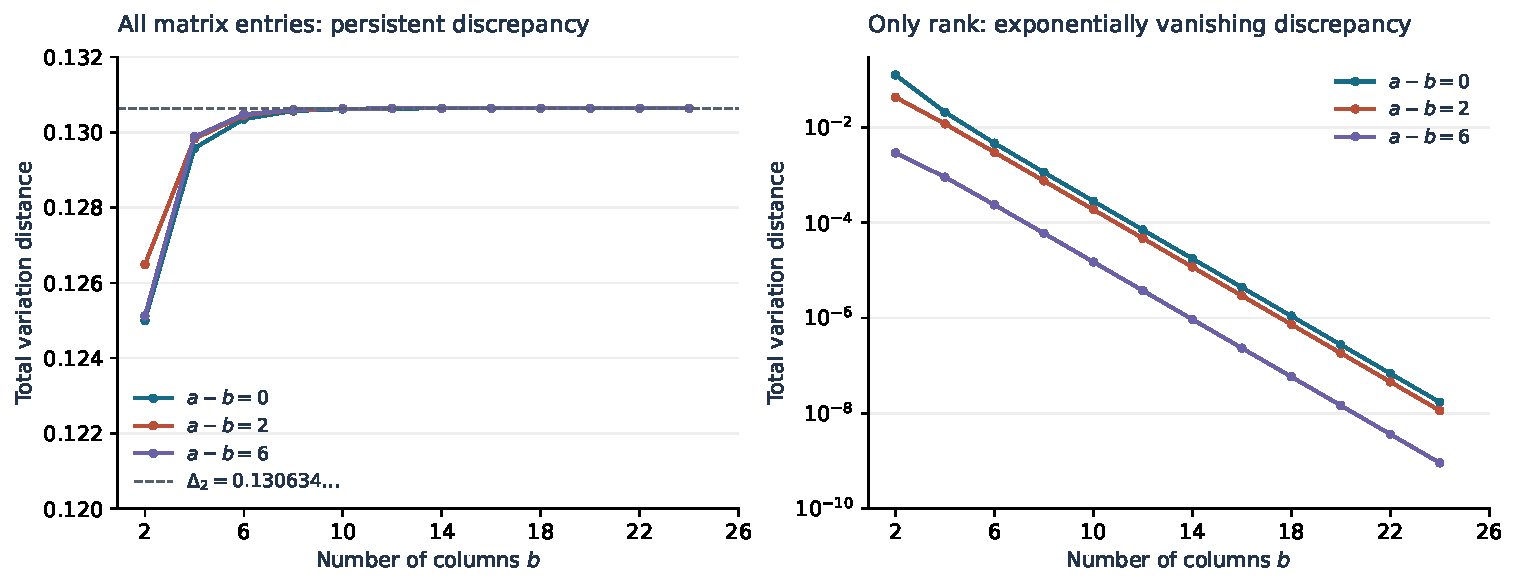
\includegraphics[width=\linewidth]{figures/rank_and_matrix_distance.pdf}
\caption{Exact finite distances over \(\mathbb F_2\), at three fixed
dimension gaps. The full-matrix distance approaches the same positive
constant; the rank distance decays exponentially. The right panel has a
logarithmic vertical scale. The figure is generated from exact fractions,
converted to floating point only for plotting.}
\label{fig:distances}
\end{figure}

\subsection{Numerical constants and verification boundary}

For a product \(\prod_{i>L}(1-t_i)\), with \(0\le t_i\le1\) and summable
\(t_i\), the elementary inequalities
\[
 1-\sum_{i>L}t_i\ \le\ \prod_{i>L}(1-t_i)\ \le\ 1
\]
give rational enclosures of each infinite product.
The supplied \path{results/constant_enclosures.json} uses 64 factors
of \(\eta\) and \(\theta\), and 128 factors of \(\gamma\), to enclose
\(\Delta_q\) for \(q=2,3,4,5\).
All printed digits of \(\Delta_2\) agree at both ends of its enclosure.
The decimal distances in the tables are rounded from exact finite
rational values; no Monte Carlo sampling is used.

The new theorems are proved in ordinary mathematical form.
They have not been formalized or checked by Lean, and inspecting the
repository's upstream formal development does not change that status.
The accompanying formalization plan separates the finite counting,
interpolation, infinite-product, and uniformity obligations.

The principal contribution is the uniform signed comparison and the
centered joint theorem. The full-distance formula is included because
it exhibits the contrast between complete data and rank statistics,
and because a published complement count independently checks it.
The fixed-positive-gap regime posed in the inspected article is
resolved for complementary nondegenerate frames. More general radical
patterns, different ambient complement dimensions, and local-ring
analogues are not treated here.



\begin{thebibliography}{9}
\raggedright
\bibitem{ProveIt}
ProveIt Contributors, \emph{ProveIt: Beyond the Riemann hypothesis for Dirichlet
\(L\)-functions: consequences, transfers and limits}, repository article,
revision \gitsha, inspected 27 November 2026.
\href{https://github.com/VladimirReshetnikov/ProveIt/blob/497c1844e71393df41914f5b783d5dc9a618eb61/Analysis/GeneralizedRiemannHypothesis/Article/sections/spn.tex}{Pinned spanning and matrix-statistics section}.

\bibitem{GRHSource}
\emph{lsernau/grh-lean}, revision
\texttt{72fead102f663d5c7a407964a13dc0cf9d977207},
as vendored in \cite{ProveIt}.
\href{https://github.com/VladimirReshetnikov/ProveIt/blob/497c1844e71393df41914f5b783d5dc9a618eb61/Analysis/GeneralizedRiemannHypothesis/vendor/grh-lean/grh/src/New/Spanning/SecondMoment/PositiveType.lean}{Positive-type functions and singular compressions}.
The present finite-field theorem does not use the analytic GRH statement.

\bibitem{FG}
J. Fulman and L. Goldstein,
\emph{Stein's method and the rank distribution of random matrices over finite fields},
Annals of Probability \textbf{43} (2015), no.~3, 1274--1314.
\href{https://doi.org/10.1214/13-AOP889}{doi:10.1214/13-AOP889};
\href{https://arxiv.org/abs/1211.0504}{arXiv:1211.0504}.

\bibitem{DBV}
M. De Boeck and G. Van de Voorde,
\emph{Anzahl theorems for trivially intersecting subspaces generating a
non-singular subspace I: symplectic and hermitian forms},
Linear Algebra and its Applications \textbf{699} (2024), 367--402.
\href{https://doi.org/10.1016/j.laa.2024.07.004}{doi:10.1016/j.laa.2024.07.004};
\href{https://arxiv.org/html/2407.07486v3}{arXiv:2407.07486v3}, Theorem~4.9.

\bibitem{PSZ}
A. Pott, K.-U. Schmidt and Y. Zhou,
\emph{Pairs of quadratic forms over finite fields},
Electronic Journal of Combinatorics \textbf{23} (2016), no.~2, P2.8.
\href{https://doi.org/10.37236/4072}{doi:10.37236/4072}.
\end{thebibliography}
\end{document}

